\makeheading{Lecture 18 | 2020-11-11}
For the $ i^{\text{th}} $ observation, the values
of its predictors are
\[ \symbf{v}_i=\begin{bmatrix}
            1 & x_{i1} & x_{i2} & \cdots & x_{i p}
      \end{bmatrix}^\top \]
\[ X=\begin{bmatrix}
            \symbf{v}_1^\top \\
            \symbf{v}_2^\top \\
            \vdots           \\
            \symbf{v}_n^\top
      \end{bmatrix} \]
\[ X^\top X=\begin{bmatrix}
            \symbf{v}_1 & \cdots & \symbf{v}_n
      \end{bmatrix}\begin{bmatrix}
            \symbf{v}_1^\top \\
            \vdots           \\
            \symbf{v}_n^\top
      \end{bmatrix}=\sum_{j=1}^{n}\symbf{v}_j\symbf{v}_j^\top \]
Recall $ H=X(X^\top X)^{-1}X^\top $ so
\[ h_{ii}=\symbf{v}_i^\top (X^\top X)^{-1}\symbf{v}_i^\top \]
Let $ X^{(i)} $ be $ X $ with $ i^{\text{th}} $ observation
deleted, $ \symbf{y}^{(i)} $ be $ \symbf{y} $ with $ i^{\text{th}} $
response deleted. Then,
\[ (X^{(i)})^{\top}X^{(i)}=\sum_{j\neq i}\symbf{v}_j\symbf{v}_j^\top
      \implies X^\top X=(X^{(i)})^\top X^{(i)}+\symbf{v}_i\symbf{v}_i^\top \]
Similarly,
\[ X^\top \symbf{y}=\sum_{j=1}^{n} \symbf{v}_j y_j\implies
      (X^{(i)})^\top \symbf{y}^{(i)}=\sum_{j\neq i}\symbf{v}_j y_j
      \implies X^{\top}\symbf{y}=(X^{(i)})^\top\symbf{y}^{(i)}+\symbf{v}_i y_i \]
Let $ A $ be an $ n\times n $ invertible matrix
\[ (A-\symbf{a}\symbf{a}^\top)^{-1}=A^{-1}+\frac{A^{-1}\symbf{a}\symbf{a}^\top
            A^{-1}}{1-\symbf{a}^\top A^{-1}\symbf{a}}  \]
Fit the least squares using $ X^{(i)} $ and $ \symbf{y}^{(i)} $
to obtain
\begin{align*}
      \hat{\symbf{\beta}}^{(i)}
       & =[(X^{(i)})^\top
      X^{(i)}]^{-1}(X^{(i)})^\top \symbf{y}^{(i)}                                                  \\
       & =(X^\top X-\symbf{v}_i\symbf{v}_i^\top)^{-1}(X^\top \symbf{y}-
      \symbf{v}_i y_i)                                                                             \\
       & =\biggl[(X^\top X)^{-1}+\frac{(X^\top X)^{-1}\symbf{v}_i\symbf{v}_i^\top
                  (X^\top X)^{-1}}{1-\symbf{v}_i^\top (X^\top X)^{-1}\symbf{v}_i} \biggr]
      (X^\top \symbf{y}-\symbf{v}_i y_i)                                                           \\
       & =(X^\top X)^{-1}X^\top\symbf{y}-(X^\top X)^{-1}\symbf{v}_i y_i+
      \frac{(X^\top X)^{-1}\symbf{v}_i\symbf{v}_i^\top (X^\top X)^{-1}X^\top\symbf{y}
      -(X^\top X)^{-1}\symbf{v}_i\symbf{v}_i^\top(X^\top X)^{-1}\symbf{v}_i y_i
      }{1-h_{ii}}                                                                                  \\
       & =\hat{\symbf{\beta}}-(X^\top X)^{-1}\symbf{v}_i
      \biggl[y_i-\frac{\symbf{v}_i^\top\hat{\symbf{\beta}}-h_{ii}y_i}{1-h_{ii}} \biggr]            \\
       & =\hat{\symbf{\beta}}-(X^\top X)^{-1}\symbf{v}_i
      \biggl[\frac{y_i-h_{ii}y_i-\symbf{v}_i^\top \hat{\symbf{\beta}}+h_{ii}y_i}{1-h_{ii}} \biggr] \\
       & =\hat{\symbf{\beta}}-(X^\top X)^{-1}\symbf{v}_i
      \biggl[\frac{y_i-\symbf{v}_i^\top \hat{\symbf{\beta}}}{1-h_{ii}} \biggr]                     \\
       & =\hat{\symbf{\beta}}-(X^\top X)^{-1}\symbf{v}_i
      \biggl[\frac{e_i}{1-h_{ii}} \biggr]                                                          \\
\end{align*}
Therefore,
\[ \hat{\symbf{\beta}}^{(i)}-\hat{\symbf{\beta}}=
      \frac{-e_i}{1-h_{ii}}(X^\top X)^{-1}\symbf{v}_i  \]
In fact, we can get $  \hat{\symbf{\beta}}^{(i)} $
from the regression with all $ n $ observations;
that is, we don't need to fit a separate model.
\begin{align*}
      D_i
       & =\frac{(\hat{\symbf{\beta}}^{(i)}-\hat{\symbf{\beta}})^{\top}
            X^\top X(\hat{\symbf{\beta}}^{(i)}-\hat{\symbf{\beta}})}{
      \hat{\sigma}^2(p+1) }                                            \\
       & =\frac{\displaystyle \biggl(\frac{-e_i}{1-h_{ii}} \biggr)
            \symbf{v}_i^\top (X^\top X)^{-1}X^\top X
            \biggl(\frac{-e_i}{1-h_{ii}} \biggr)(X^\top X)^{-1}\symbf{v}_i}{
            \hat{\sigma}^2(p+1)
      }                                                                \\
       & =\frac{e_i^2}{\hat{\sigma}^2(1-h_{ii})(1-h_{ii})}
      \biggl(\frac{h_{ii}}{p+1} \biggr)                                \\
       & =d_i^2\biggl(\frac{h_{ii}}{1-h_{ii}} \biggr)
      \biggl(\frac{1}{p+1} \biggr)
\end{align*}
as claimed, so we can calculate Cook's distance in terms of
$ \abs{d_i} $ and $ h_{ii} $. Therefore, the most influential
observation on estimates of $ \symbf{\beta} $
are those with high $ \abs{d_i} $ and $ h_{ii} $.
\subsection{R Demo}
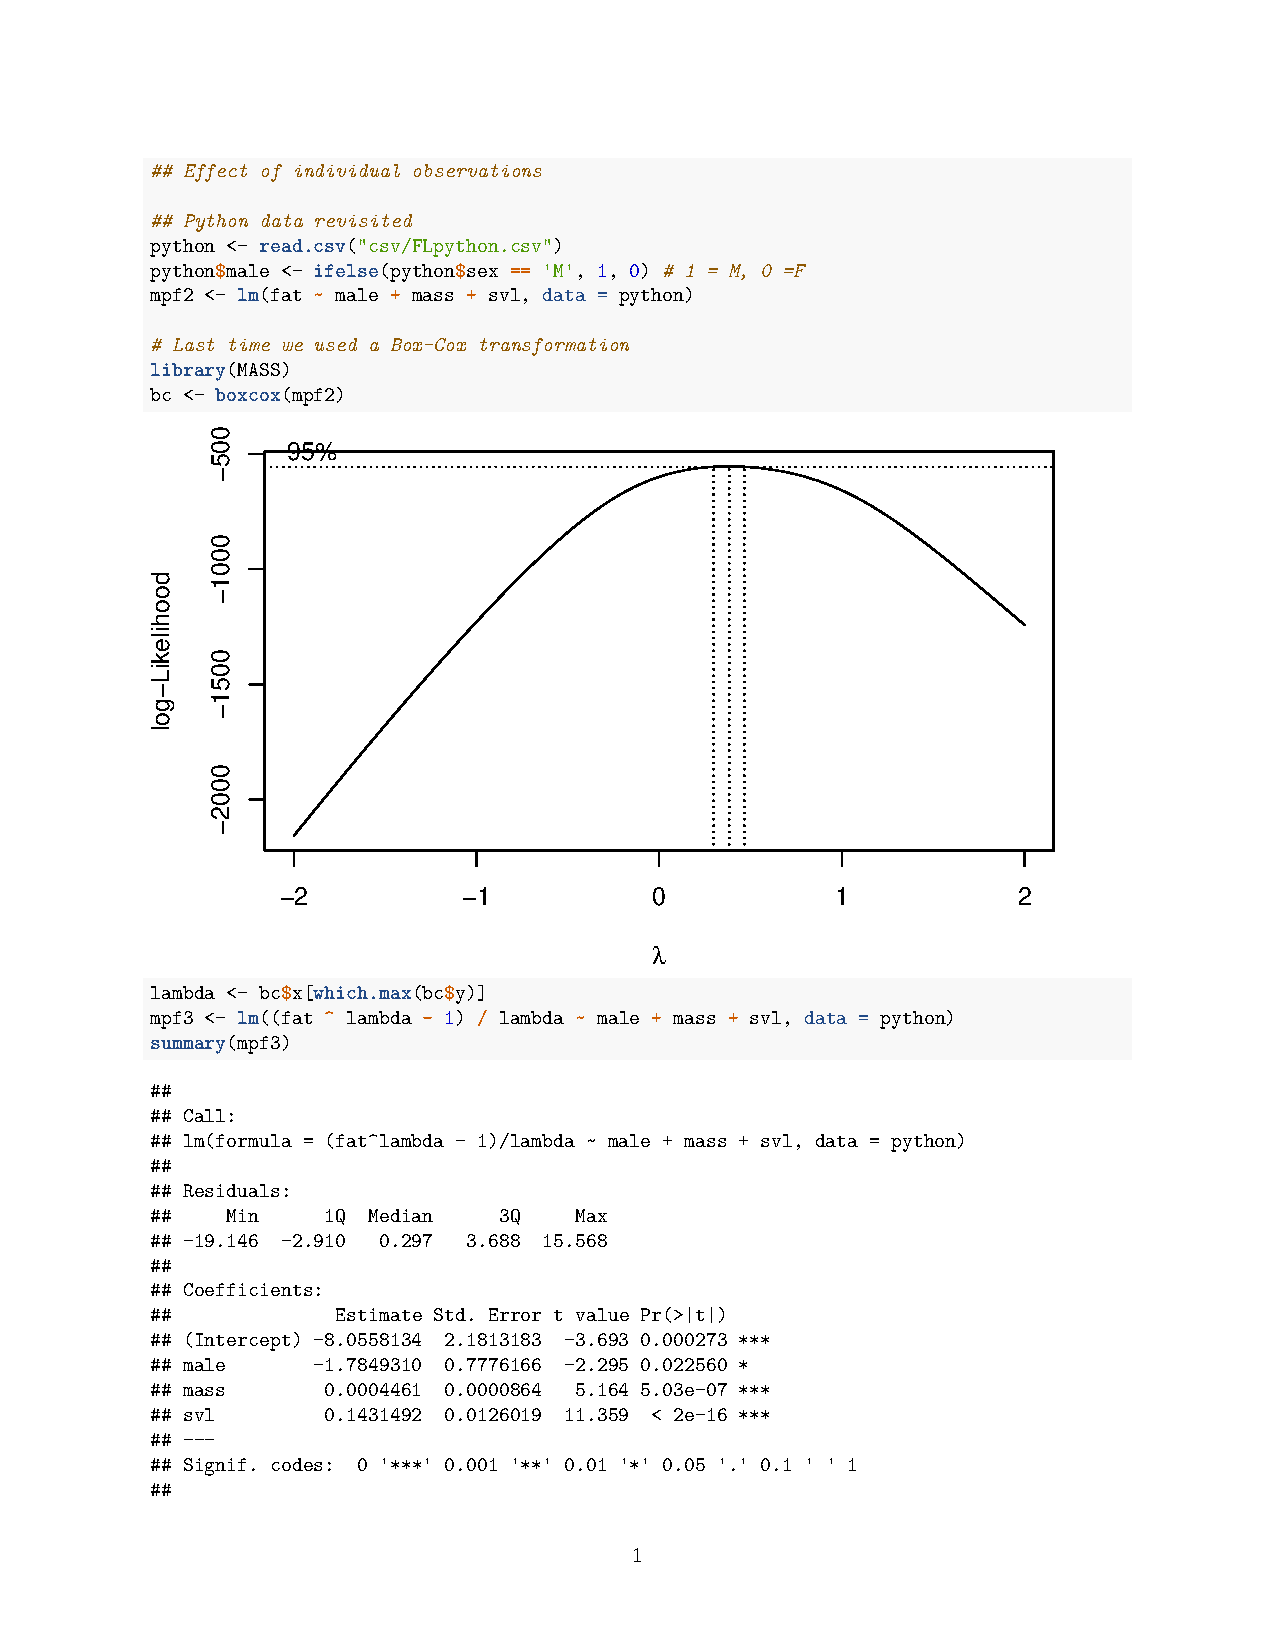
\includepdf[pages=-]{lec_18-demo.pdf}
